% !TeX spellcheck = cs_CZ
\documentclass{beamer}
\usepackage[orientation=portrait,size=us0,scale=1.2,debug]{beamerposter}
%\mode<presentation>
\newcommand{\faculty}{DFJP}															% select theme according to the UPa faculty (DFJP,FEI,FCHT,FES,FR,FZS,FF,UPA)
\newcommand{\footlineleft}{https://dfjp.upce.cz/}									% insert footer left content here
\newcommand{\footlinecenter}{2. a 3. prosince 2020}									% insert footer center content here
\newcommand{\footlineright}{petr.vnenk@upce.cz}										% insert footer right content here
\usetheme{UPA}
\usepackage{chemformula}
\usepackage[utf8]{inputenc}
\usepackage{csquotes}																% enable Czech quotation marks
\usepackage[english, czech]{babel}													% required for rendering special characters
\usepackage{hyperref} 																% enable hyperlink for urls
\usepackage{ragged2e}
\usepackage[
backend=biber															% !!! --->	% set biber instead of BibTex into compilator!
,style=iso-numeric
,sortlocale=cs_CZ														% !!! --->	% set local language environment ("cs_CZ" for Czech)!
,autolang=other
,bibencoding=UTF8
]{biblatex}																			% extended options of bibliography management
\addbibresource{bib.bib}												% !!! --->	% bibliography source file (modify according to your needs)
\usepackage[font=scriptsize,justification=justified]{caption}
\usepackage{array,booktabs,tabularx}

\newcolumntype{Z}{>{\centering\arraybackslash}X} 									% centered tabularx columns

\title{\huge Vyhodnocení zbytkové a průměrné životnosti udržovaných silničních mostů}
\author{Petr Vnenk$^{1}$, Özgür Yurdakul$^{1}$, Dušan Chocholouš$^{2}$}
\institute{$^{1}$Dopravní fakulta Jana Pernera, Univerzita Pardubice \\ $^{2}$Správa a údržba silnic Pardubického kraje}
\date{\today}

% edit this depending on how tall your header is. We should make this scaling automatic :-/
\newlength{\columnheight}
\setlength{\columnheight}{107 cm}

\begin{document}
\begin{frame}
\begin{columns}
	\begin{column}{.4\textwidth}
		\begin{beamercolorbox}[center]{postercolumn}
			\begin{minipage}{.98\textwidth}  % tweaks the width, makes a new \textwidth
				\parbox[t][\columnheight]{\textwidth}{ % must be some better way to set the the height, width and textwidth simultaneously
					\begin{myblock}{Abstrakt}
						Visuální mostní prohlídky poskytují hodnotná a~často aktualizovaná data, která mohou snadno sloužit jako zdroj informací pro správce mostů a~osoby v~rozhodujících pozicích samospráv. Úroveň degradace částí mostů je zjišťována pravidelnými visuálními prohlídkami. Na základě klasifikačního stupně celkového stavu mostní konstrukce anebo klasifikačních stupňů jednotlivých částí mostní konstrukce je prováděna nezbytná a~preventivní údržba. Kromě uvedených možností využití lze z~dat z~mostních prohlídek za použití vhodných modelů vypočítat zbytkovou a~průměrnou životnost mostů a~optimalizovat alokaci zdrojů pro údržbu. V~tomto článku je diskutována zjednodušená metodika určování zbytkové a~průměrné životnosti mostů na základě dat z~mostních prohlídek využívající lineární regresi. Teoretický rozbor je doplněn aplikací na vzorku 50~mostů v~okresech Chrudim a~Pardubice. Při aplikaci této metodiky předpokládající rovnoměrnou rychlost degradace všech mostů (tj.~lineární regrese) je vypočtená průměrná doba životnosti 88~let.
					\end{myblock}\vfill
					\begin{myblock}{O~životnosti mostů řečí čísel}
						\begin{figure}
							\centering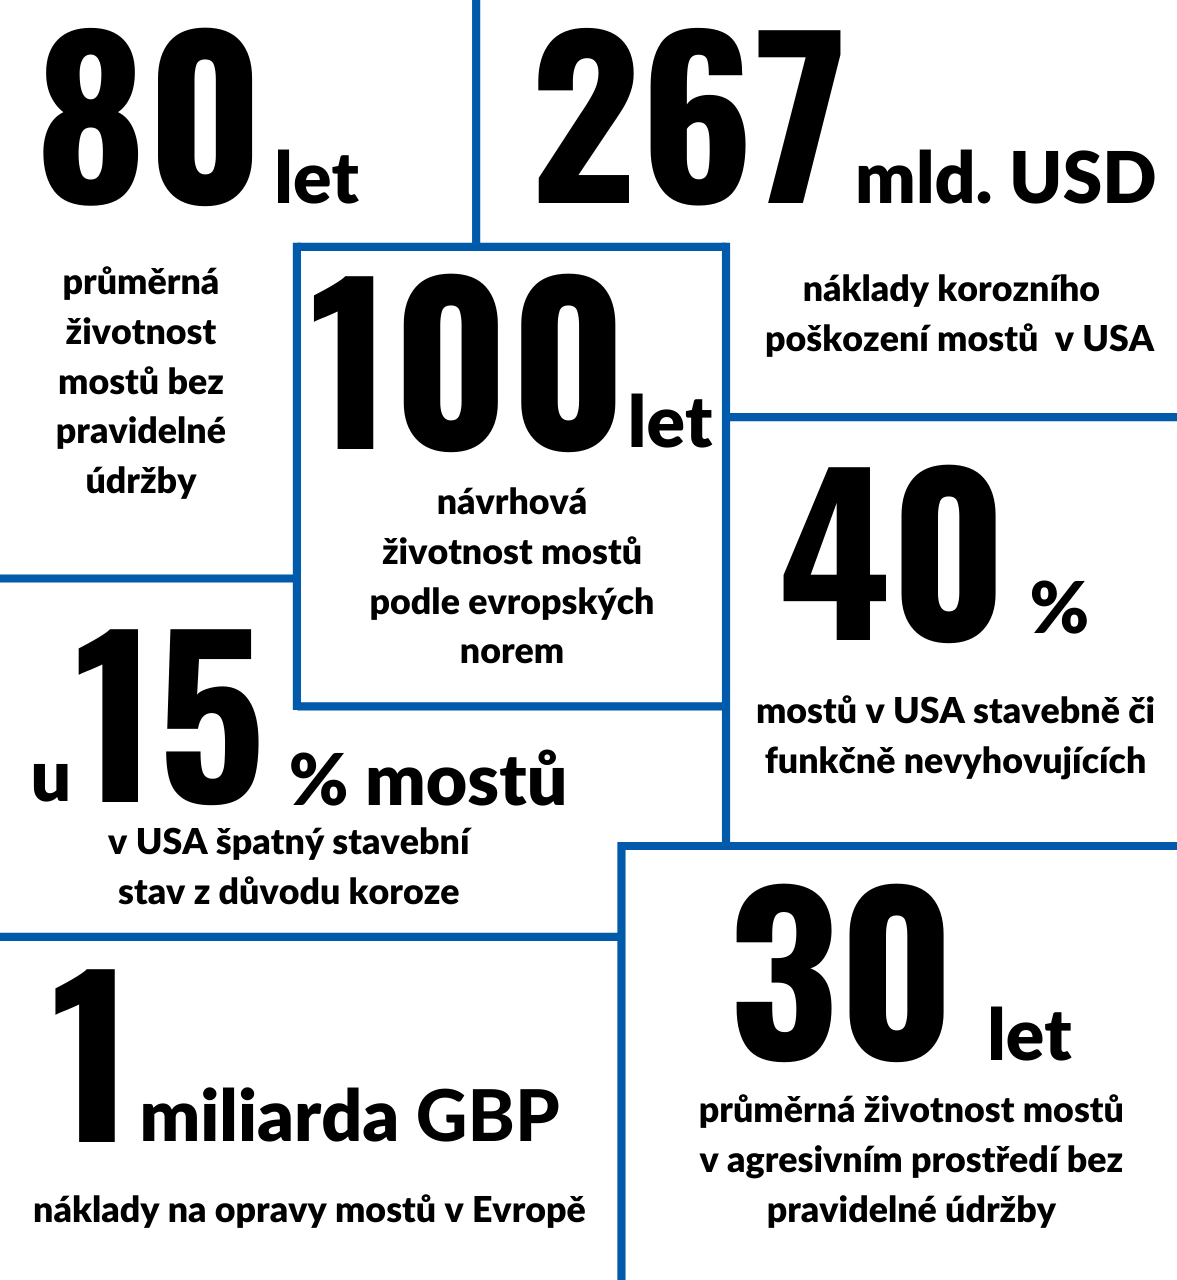
\includegraphics[width=0.99\textwidth]{img/poster3}
							\label{fig:poster3}
						\end{figure}
					\end{myblock}\vfill
					\begin{myblock}{Metodika}
						Studie byla provedena na reprezentativním vzorku betonových silničních mostů
						\vskip 0.2cm
						\begin{itemize}
							\item na silnicích I., II. a~III.~třídy,
							\item o~délce alespoň 5~m,
							\item v~okresech Pardubice a~Chrudim.
						\end{itemize}
						\vskip 0.5cm
						Z~toho důvodu bylo všech 228~mostů ve zmíněných okresech nejprve roztřízeno podle
						\vskip 0.2cm
						\begin{itemize}
							\item typu konstrukce,
							\item statického působení,
							\item počtu polí,
						\end{itemize}
						\vskip 0.2cm
						a~dále byl sestaven histogram četnosti výskytu jednotlivých kategorií mostů v~okresech. Těchto 228~mostů bylo dále redukováno na 50 pro účely mostních prohlídek, přičemž byla respektována proporcionalita mostů na silnicích I., II. a~III. třídy a~každého typu konstrukce. 
						\vskip 0.5cm
						Při výběru mostů do reprezentativních vzorků byla dále použita kritéria
						\vskip 0.2cm
						\begin{enumerate}
							\item stáří mostu,
							\item stavební stav mostu.
						\end{enumerate}
						\vskip 0.4cm
						Mosty byly podle každého z~těchto kritérií vybírány tak, aby byly rozdílné hodnoty zastoupeny rovnoměrně (tj.~bylo-li třeba vybrat 4~mosty ze 7 v~rámci jedné kategorie, mosty byly seřazeny podle stáří a~vybrán byl 1., 3., 5.~a~7.~most).
						\begin{figure}
							\centering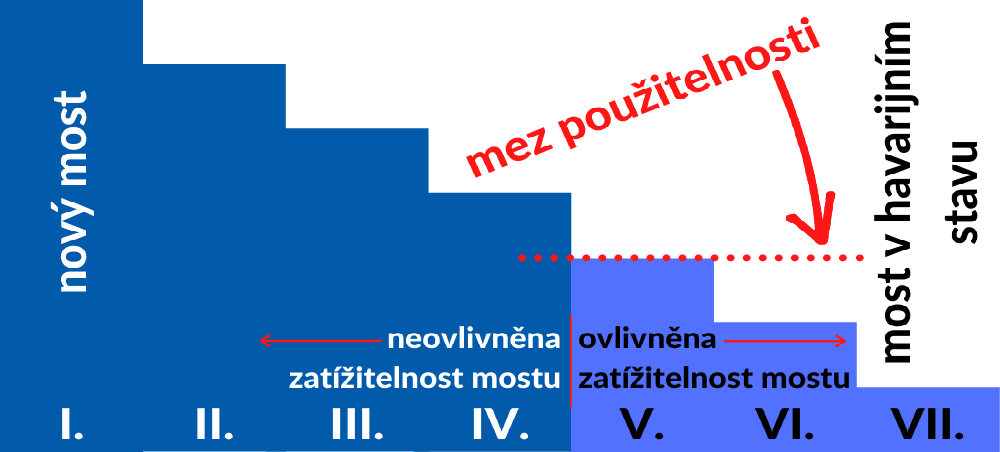
\includegraphics[width=0.9\textwidth]{img/stupne}
							\caption{Stupně stavebního stavu mostu podle ČSN 73 6221.}
							\label{fig:stupne}
						\end{figure}
					\end{myblock}\vfill
		}\end{minipage}\end{beamercolorbox}
	\end{column}
	\begin{column}{.60\textwidth}
		\begin{beamercolorbox}[center]{postercolumn}
			\begin{minipage}{.98\textwidth} % tweaks the width, makes a new \textwidth
				\parbox[t][\columnheight]{\textwidth}{ % must be some better way to set the the height, width and textwidth simultaneously
					\begin{myblock}{Reprezentativní vzorek}
						\vskip 0.4cm
						\begin{figure}
							\begin{minipage}{0.4\textwidth}
								\centering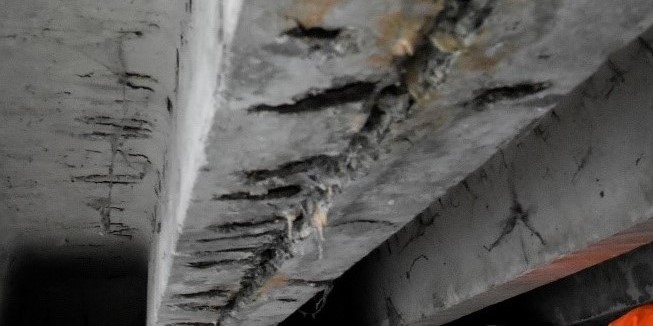
\includegraphics[width=1\textwidth]{img/1a}
								\caption*{(a)}
							\end{minipage}
							\hspace{1em}
							\begin{minipage}{0.4\textwidth}
								\centering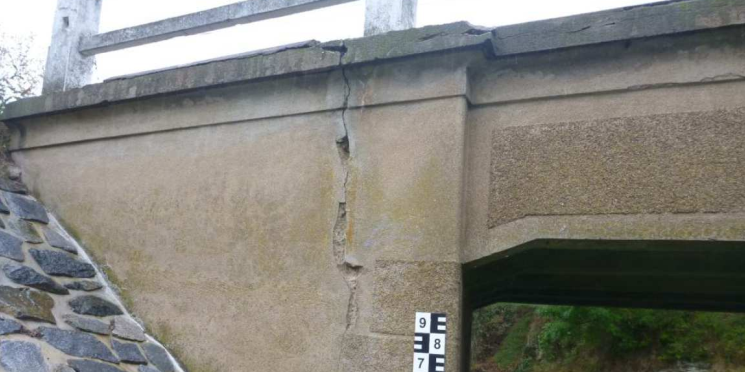
\includegraphics[width=1\textwidth]{img/1b}
								\caption*{(b)}
							\end{minipage}
							\vskip 0.5cm
							\begin{minipage}{0.4\textwidth}
								\centering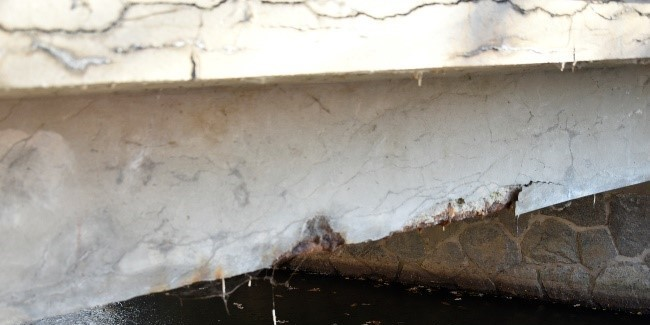
\includegraphics[width=1\textwidth]{img/1c}
								\caption*{(c)}
							\end{minipage}
							\hspace{1em}
							\begin{minipage}{0.4\textwidth}
								\centering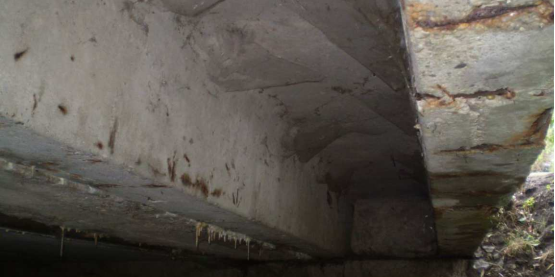
\includegraphics[width=1\textwidth]{img/1d}
								\caption*{(d)}
							\end{minipage}
							\caption{Degradace částí prohlížených mostů: (a) 3237-2, (b) 35815-1, (c) 34039-2, (d) 3237-1.}
						\end{figure}
						\vskip 0.5cm
						\begin{minipage}{1\textwidth}
							\begin{columns}
								\begin{column}{0.72\textwidth}
									\begin{figure}
										\begin{minipage}{0.9\textwidth}
											\centering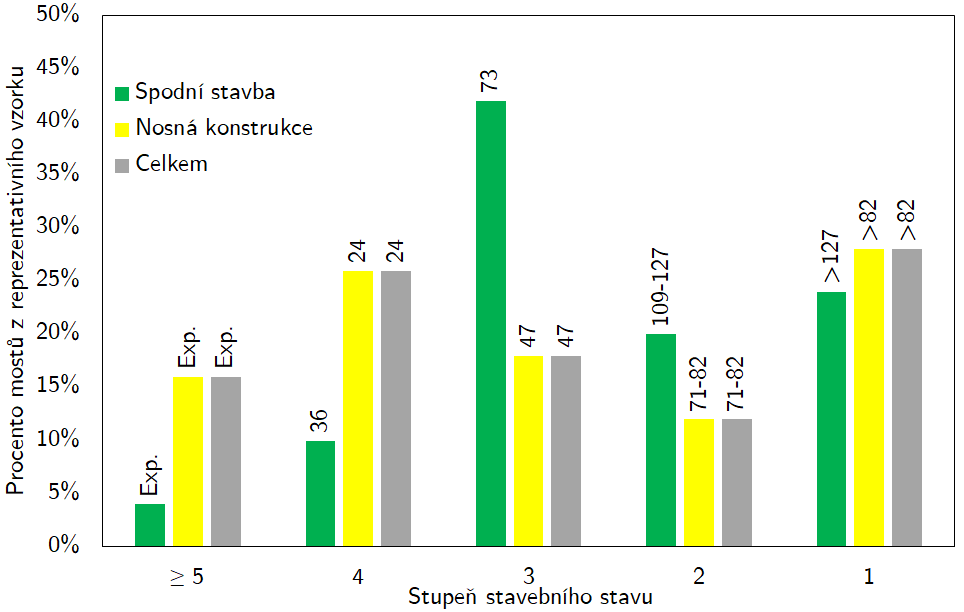
\includegraphics[width=1\textwidth]{img/2}
											\caption{Zbytková životnost mostů získaná lineární analýzou.}
											\label{fig:fail2}
										\end{minipage}
									\end{figure}
								\end{column}
								\begin{column}{0.28\textwidth}
									\begin{minipage}{0.9\textwidth}
										Predikce míry degradace a~vývoje rychlosti degradace mostní konstrukce v~čase jsou náročnými úlohami, skrze pravidelné mostní prohlídky však mohou být zjištěny. Pravidelná údržba a~přijatá opatření udržují stav mostu na určité úrovni, existují však i~mosty, jejichž stupeň stavebního stavu mez použitelnosti už překročil a~stavební úprava je nezbytná pro obnovu jejich použitelnosti. V~celkovém hodnocení stavebního stavu tvoří převážnou většinu mosty na stupni IV a~I (obrázek 2).
									\end{minipage}
								\end{column}
							\end{columns}
						\end{minipage}
					\end{myblock}\vfill
					\begin{myblock}{Výsledky a~diskuse}
						V~této studii je určena zbytková životnost mostů metodou založenou na údajích z~mostních prohlídek a~statistické analýze.
						\vskip 1cm
						\begin{itemize}
							\item Byla použita zjednodušená metoda určování zbytkové životnosti mostů počítající s~rovnoměrnou rychlostí degradace.
							\item Byl sestrojen graf závislosti jednotlivých stavebních stavů mostů na jejich stáří.
							\item Tímto grafem byla proložena přímka sestrojená metodou nejmenších čtverců.
						\end{itemize}
						\vskip 1cm
						Vztah hodnocení stupně stavebního stavu mostu a~jeho stáří byl sestaven pro hodnocení spodní stavby, nosné konstrukce a~pro celkové hodnocení konstrukce. Pro určení očekávané životnosti mostů byla použita lineární regrese. Zbytková životnost je spočítána podle rovnice, která zahrnuje předpoklad vývoje životnosti mostu s~rovnoměrnou rychlostí degradace.
						\vskip 0.1cm
						\begin{equation*}
							R_{TL} = \frac{5 - C_{TL}}{M_{TL}}
						\end{equation*}
						\vskip 0.5cm
						kde $ R_{TL} $ je zbytková životnost, $ C_{TL} $ je aktuální stupeň stavebního stavu a~$ M_{TL} $ je rychlost degradace (tj.~směrnice přímky).
						\vskip 1cm
						\begin{figure}
							\begin{minipage}{0.30\textwidth}
								\centering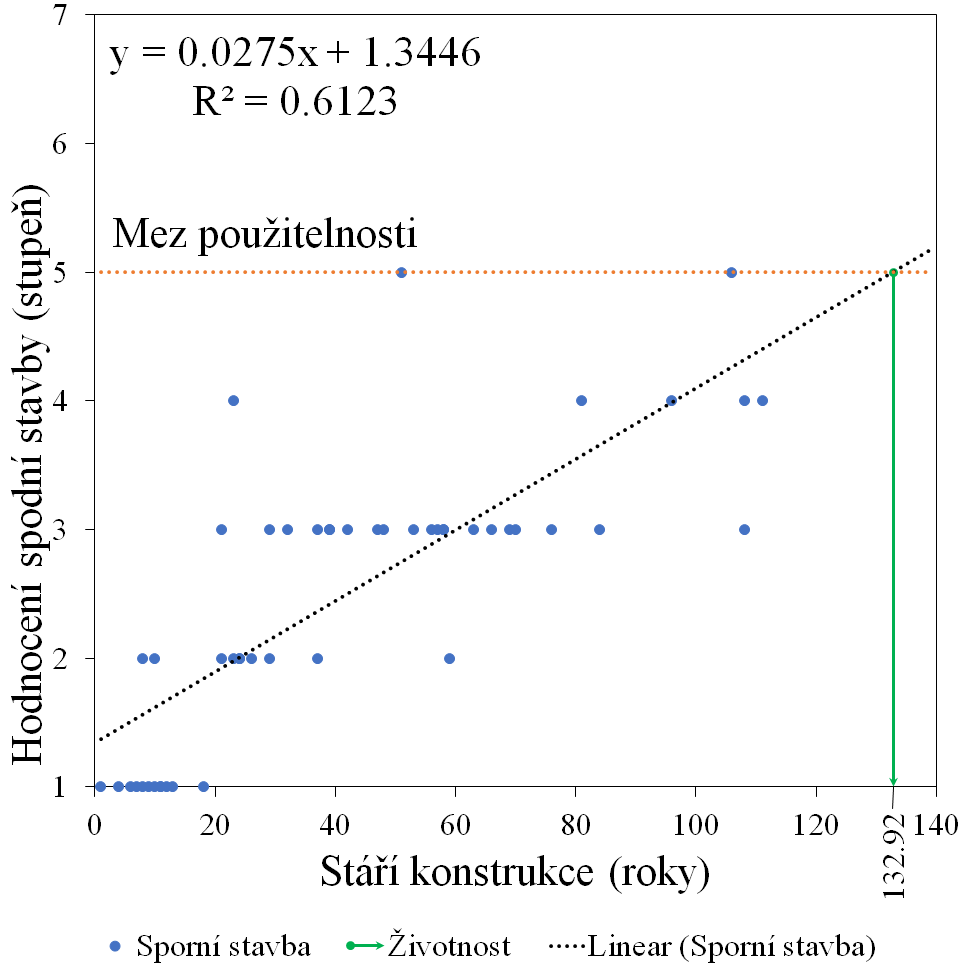
\includegraphics[width=1\textwidth]{img/3a}
								\caption*{(a)}
							\end{minipage}
							\hspace{1em}
							\begin{minipage}{0.30\textwidth}
								\centering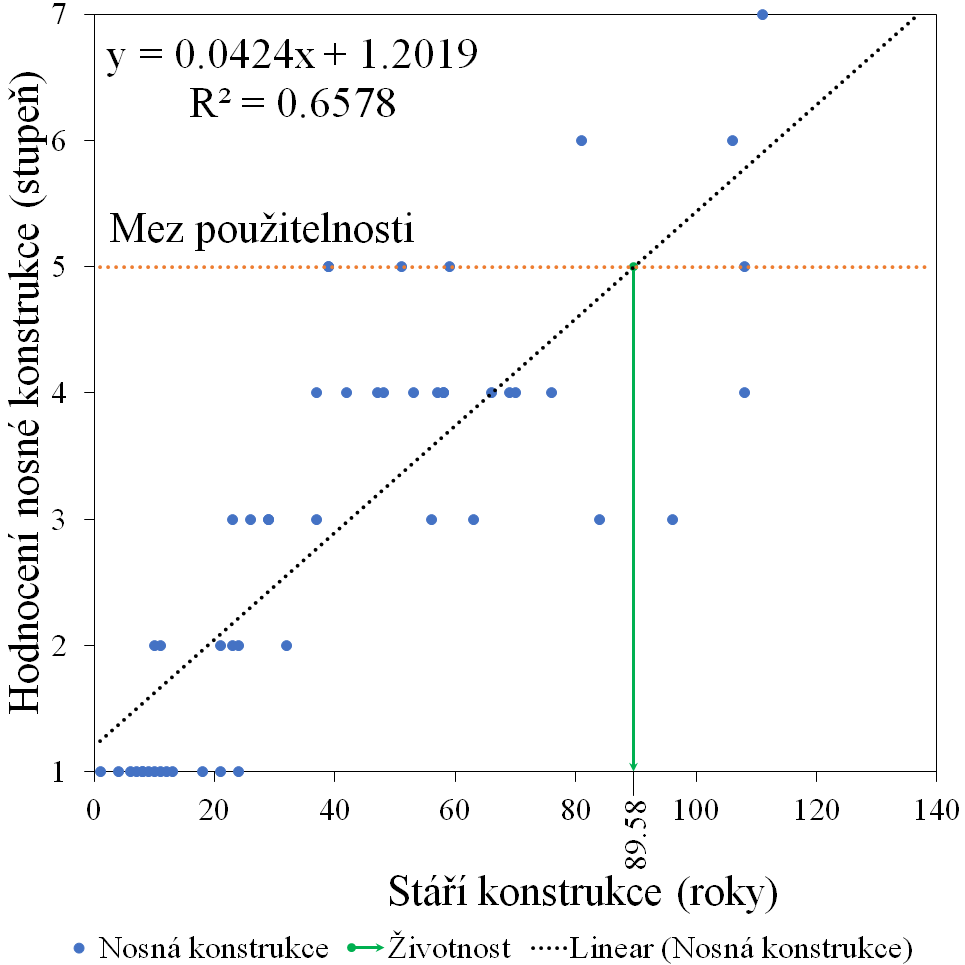
\includegraphics[width=1\textwidth]{img/3b}
								\caption*{(b)}
							\end{minipage}
							\hspace{1em}
							\begin{minipage}{0.30\textwidth}
								\centering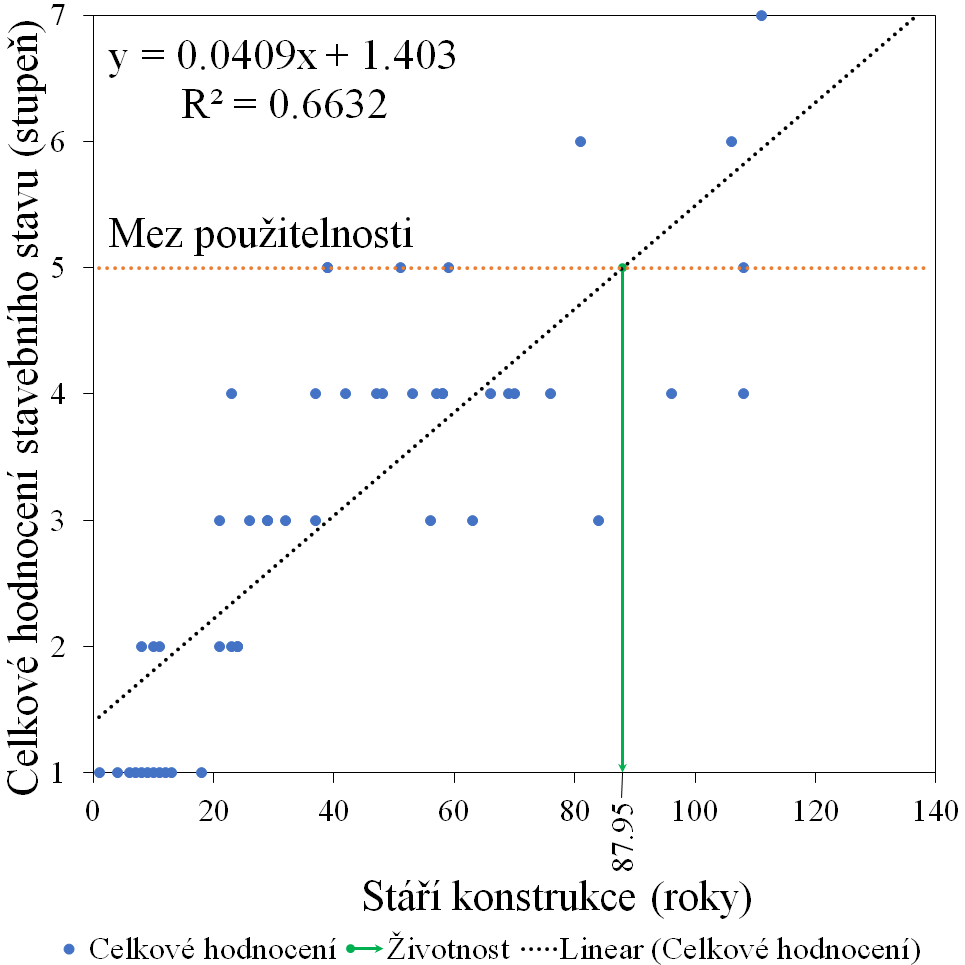
\includegraphics[width=1\textwidth]{img/3c}
								\caption*{(c)}
							\end{minipage}
							\caption{Aktuální stav mostů s~proloženou přímkou degradace: (a) spodní stavba, (b) nosná konstrukce, (c) celkové hodnocení mostů.}
						\end{figure}
						Návrhová životnost mostu 100~let nebyla lineární regresí pro celkové hodnocení dosažena. Průměrná životnost do dosažení meze použitelnosti při celkovém hodnocení stavebního stavu konstrukce je 87,95~roku, což je zhruba o~12~let méně, než návrhová hodnota. Také průměrná životnost do dosažení meze použitelnosti nosné konstrukce je nižší, a~to 89,58~roku. Naopak průměrná životnost spodní stavby je se 133~lety výrazně vyšší než návrhová, což značí trvanlivější konstrukce.
					\end{myblock}\vfill
					\begin{myblock}{Závěr}
						Cílem této práce je přispět k diskusi o~určování zbytkové životnosti silničních mostů z~dat z~mostních prohlídek. Tato data tvoří praktickou databázi, neboť mostní prohlídky jsou jednou ze základních činností správců mostní infrastruktury. Byla představena zjednodušená metodika určování zbytkové životnosti mostů. Teoretický postup byl aplikován na reprezentativní vzorek 50~mostů, u~nichž byla zbytková životnost stanovena a~výsledky diskutovány. Dále jsou diskutovány průměrné životnosti spodní stavby, nosné konstrukce a~mostů jako celku. Tato analýza může správcům mostní infrastruktury indikovat, jaké mosty, potažmo jejich části vykazují zvýšenou míru degradace a~jaká je životnost mostů ve vyšetřované oblasti. Uvedená metodika může pomoci optimalizovat údržbu mostů a~také odpovědně alokovat zdroje pro jejich údržbu.
					\end{myblock}\vfill
		}\end{minipage}\end{beamercolorbox}
	\end{column}
\end{columns}
\end{frame}
\end{document}
